\section*{Question 2}
\subsection{Équations du mouvement}
Intéressons nous maintenant au cas où les deux corps sont de masse similaire. L'Hamiltonien du système doit bien entendu être redéfini, il est maintenant donné par 

$$\Ha(p_1,p_2,q_1,q_2) = \frac{1}{2} (\frac{1}{m_1} p_1^T p_1 + \frac{1}{m_2} p_2^T p_2) - G \frac{m_1 m_2}{||q_1- q_2||_2} $$

où $G$ représente la constante gravitationnelle et $m_i$ ma masse du corps $i$. On garde les mêmes conventions qu'à la question 1, c'est à dire que 
 $$q =
\begin{pmatrix}
  q_1\\
  q_2
\end{pmatrix}$$,
$$p =
\begin{pmatrix}
  p_1\\
  p_2
\end{pmatrix}$$ et
$f_1(q,p)$ et $f_2(q,p)$ sont tels que
\begin{align*}
  \dot{q} & = f_1(p,q)\\
  \dot{p} & = f_2(p,q).
\end{align*}

On calcule, en se rappelant des résultats de la question 1 mais en n'oubliant cependant pas d'inclure les masses 
 
\begin{align*}
 f_{1,i}(q,p) &= m_i \fpart{\Ha(p,q)}{p_i} \\	
  f_1(p) & =
  \begin{pmatrix}
    m_1\frac{p_1}{m_1}\\
    m_2\frac{p_2}{m_2}
  \end{pmatrix}\\
  & = p\\
%	
 f_{2,i}(q,p) &= -\frac{1}{m_i}\fpart{\Ha(p,q)}{q_i} \\
  f_2(q) & = Gm_1m_2
  \begin{pmatrix}
    \frac{-q_1}{m_1\|q_1-q_2\|_2^3}\\
    \frac{q_2}{m_2\|q_1-q_2\|_2^3}
  \end{pmatrix}\\
  & = G
  \begin{pmatrix}
    \frac{-m_2q_1}{\|q_1-q_2\|_2^3}\\
    \frac{m_1q_2}{\|q_1-q_2\|_2^3}
  \end{pmatrix}.
\end{align*}

\begin{figure}
  \centering
  \begin{subfigure}[b]{0.3\textwidth}
    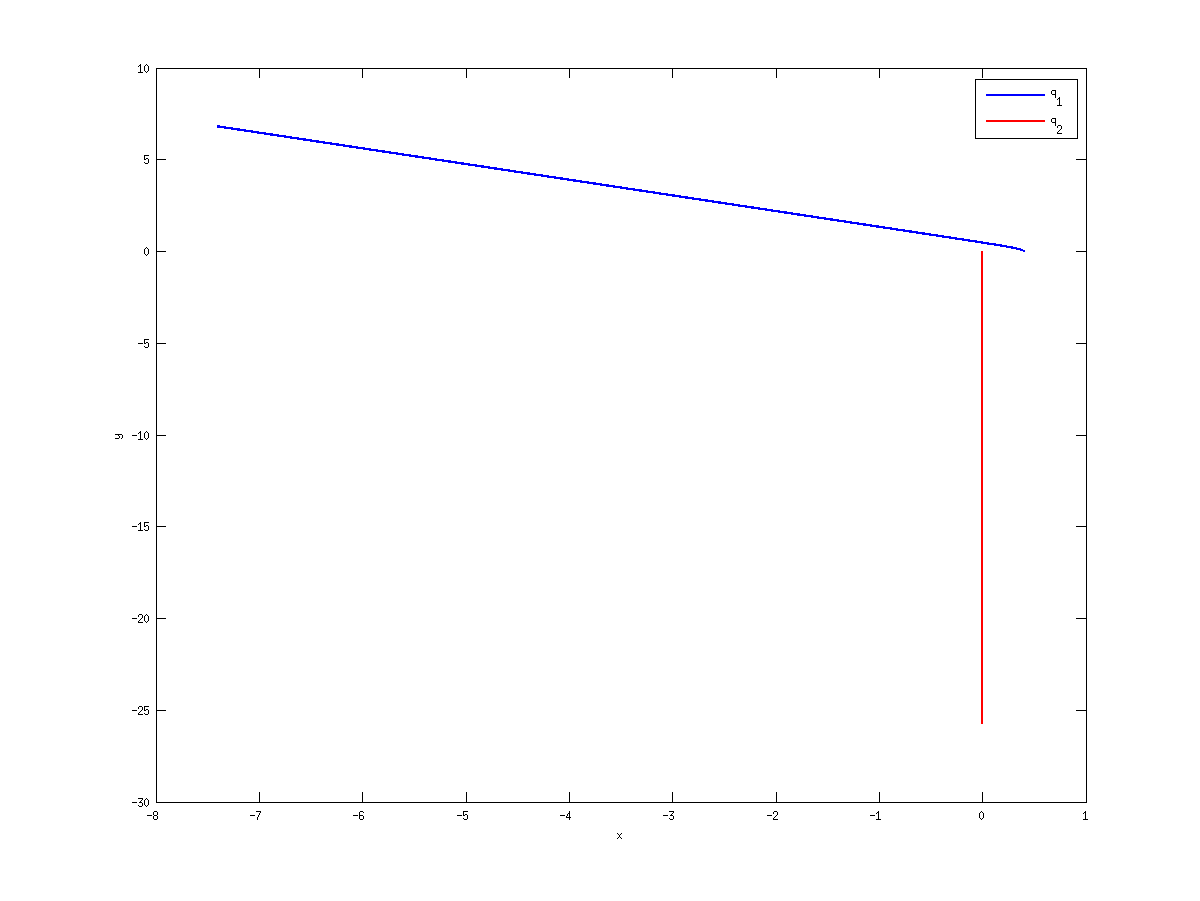
\includegraphics[width=\textwidth]{images/Q2_explicite_q.png}
    \caption{$q$ pour explicite}
    \label{fig:q2_explicite_q}
  \end{subfigure}%
  ~ %add desired spacing between images, e. g. ~, \quad, \qquad etc.
  %(or a blank line to force the subfigure onto a new line)
  \begin{subfigure}[b]{0.3\textwidth}
    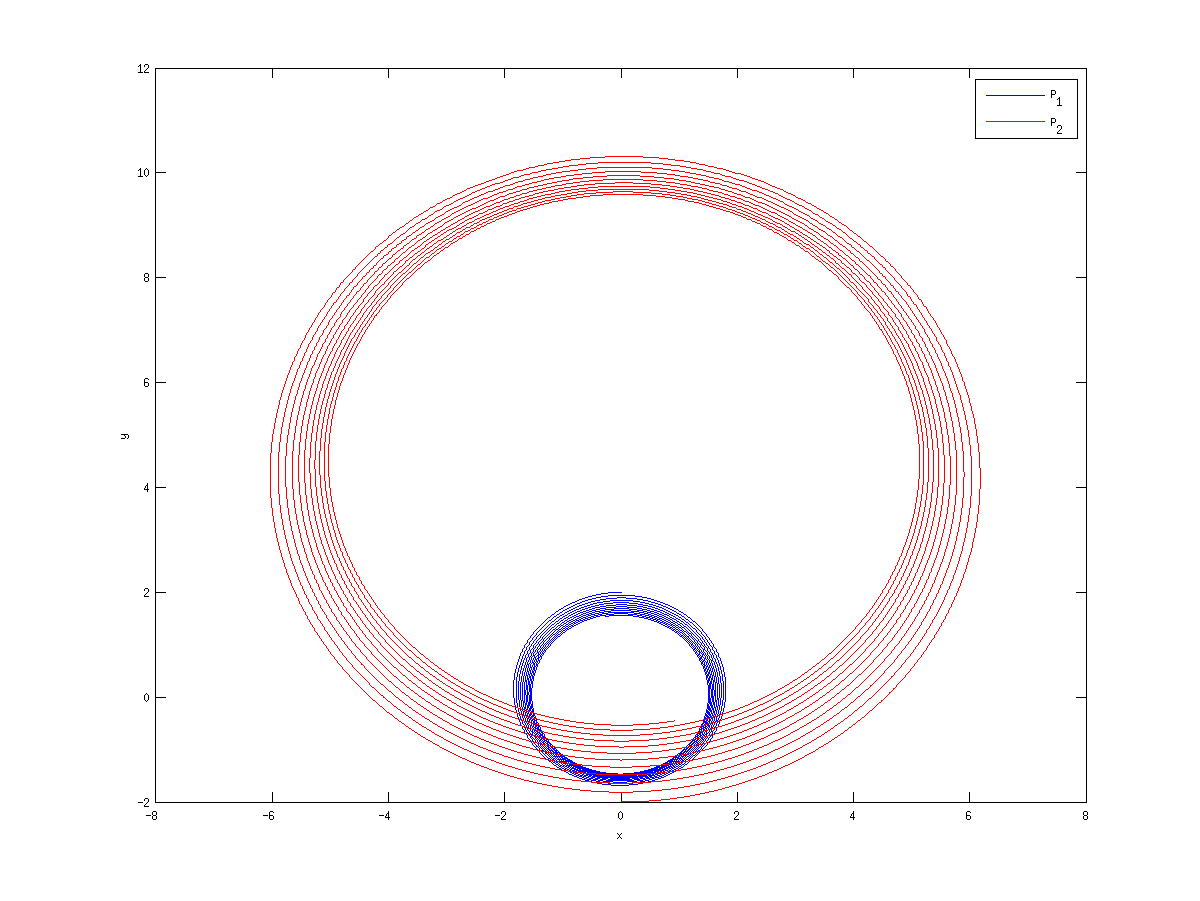
\includegraphics[width=\textwidth]{images/Q2_explicite_p.png}
    \caption{$p$ pour explicite}
    \label{fig:q2_explicite_p}
  \end{subfigure}
  ~
  \begin{subfigure}[b]{0.3\textwidth}
    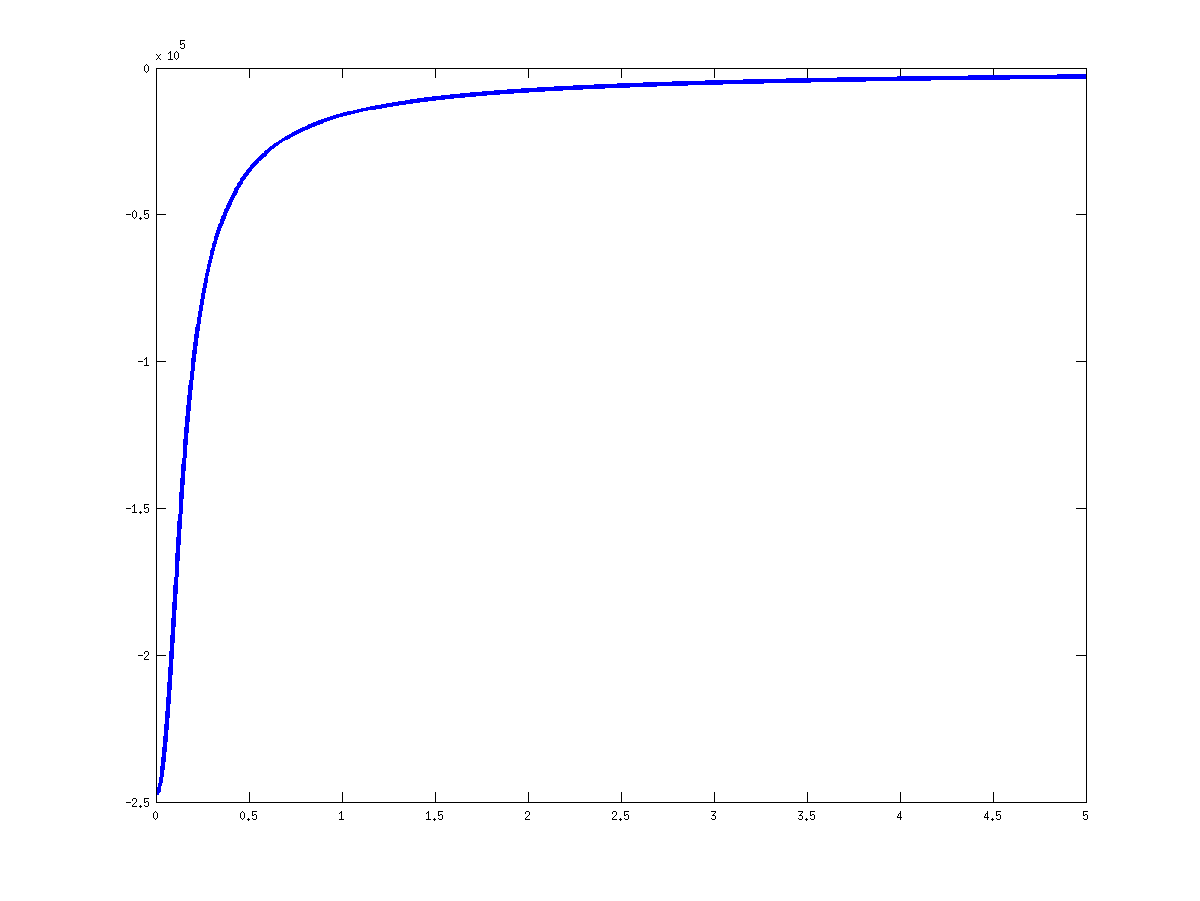
\includegraphics[width=\textwidth]{images/Q2_explicite_H.png}
    \caption{$\Ha$ pour explicite}
    \label{fig:q2_explicite_H}
  \end{subfigure}

  \begin{subfigure}[b]{0.3\textwidth}
    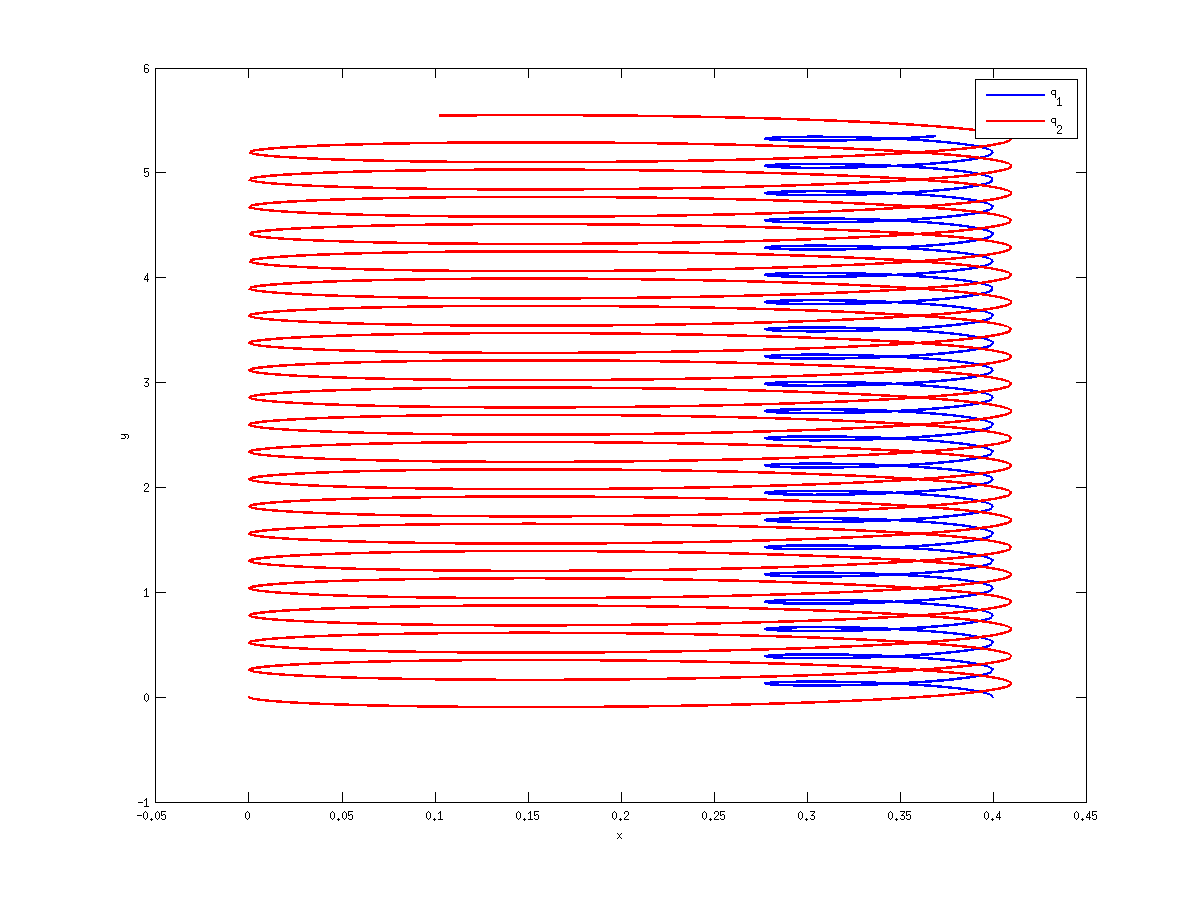
\includegraphics[width=\textwidth]{images/Q2_symplectique1_q.png}
    \caption{$q$ pour symplectique1}
    \label{fig:q2_symplectique1_q}
  \end{subfigure}%
  ~
  %(or a blank line to force the subfigure onto a new line)
  \begin{subfigure}[b]{0.3\textwidth}
    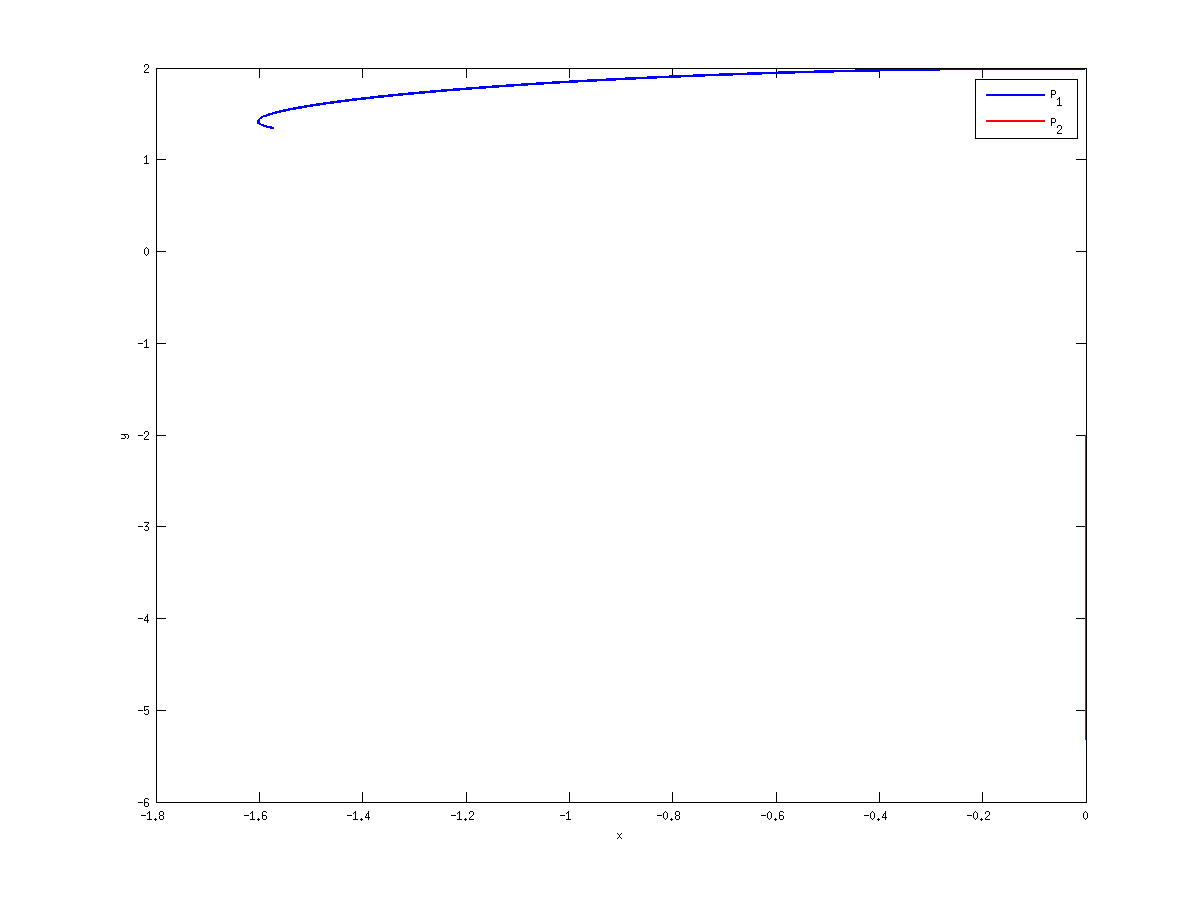
\includegraphics[width=\textwidth]{images/Q2_symplectique1_p.png}
    \caption{$p$ pour symplectique1}
    \label{fig:q2_symplectique1_p}
  \end{subfigure}
  ~
  \begin{subfigure}[b]{0.3\textwidth}
    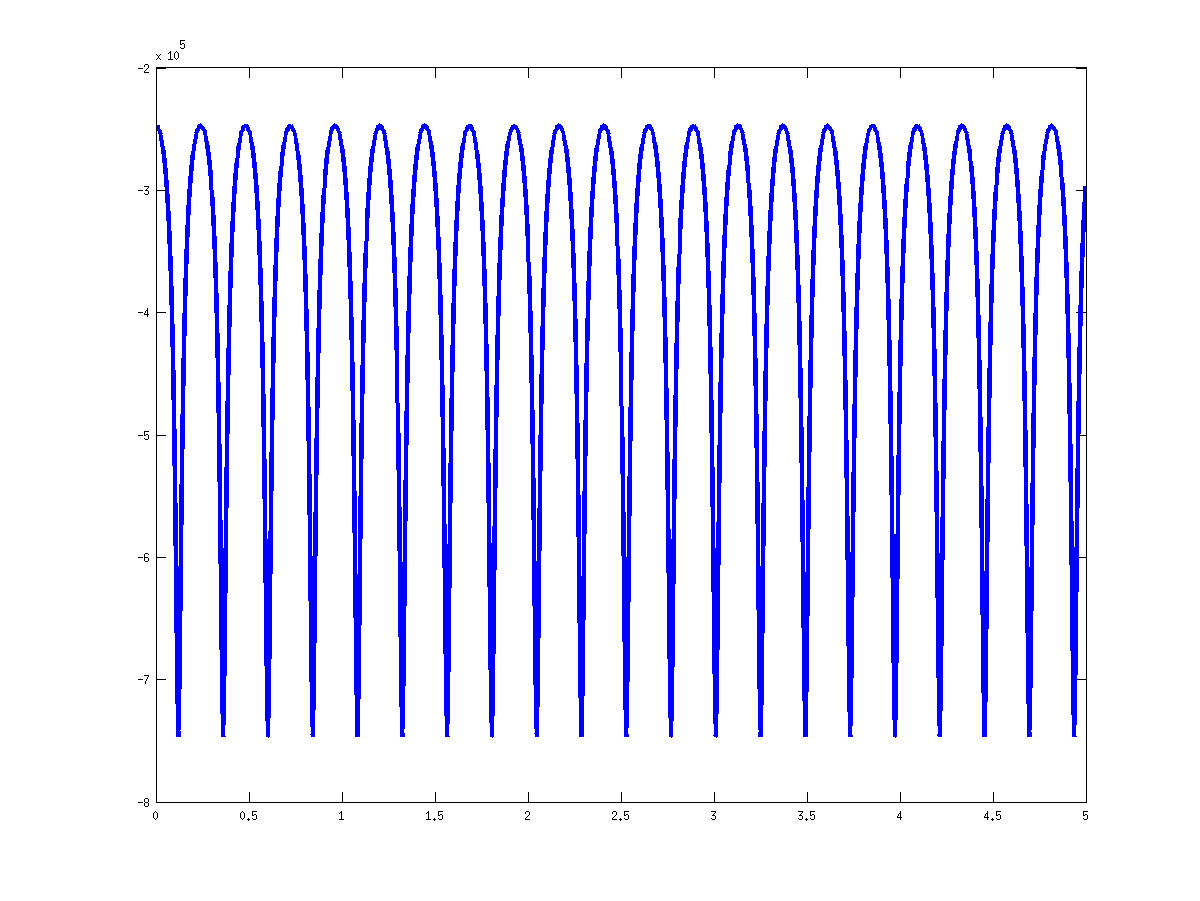
\includegraphics[width=\textwidth]{images/Q2_symplectique1_H.png}
    \caption{$\Ha$ pour symplectique1}
    \label{fig:q2_symplectique1_H}
  \end{subfigure}

  \begin{subfigure}[b]{0.3\textwidth}
    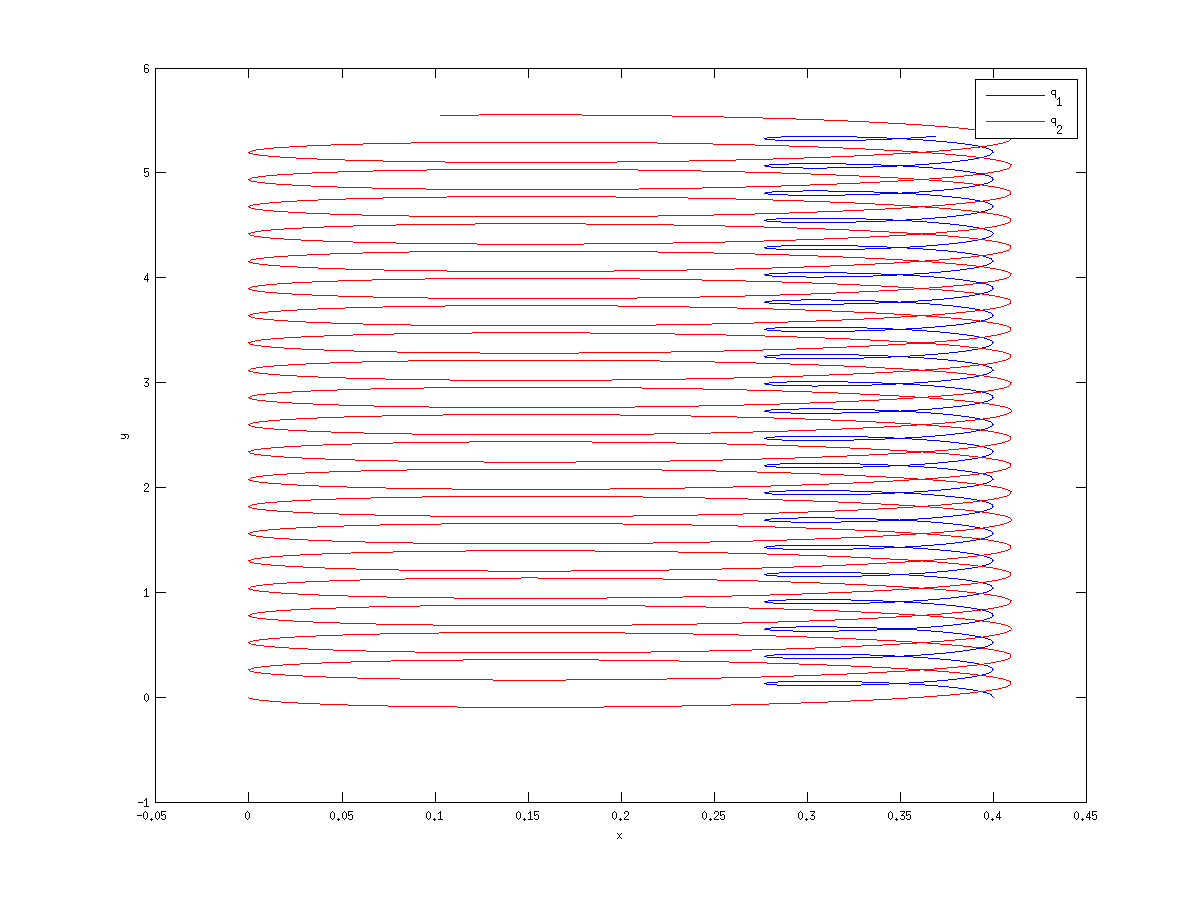
\includegraphics[width=\textwidth]{images/Q2_symplectique2_q.png}
    \caption{$q$ pour symplectique2}
    \label{fig:q2_symplectique2_q}
  \end{subfigure}%
  ~
  %(or a blank line to force the subfigure onto a new line)
  \begin{subfigure}[b]{0.3\textwidth}
    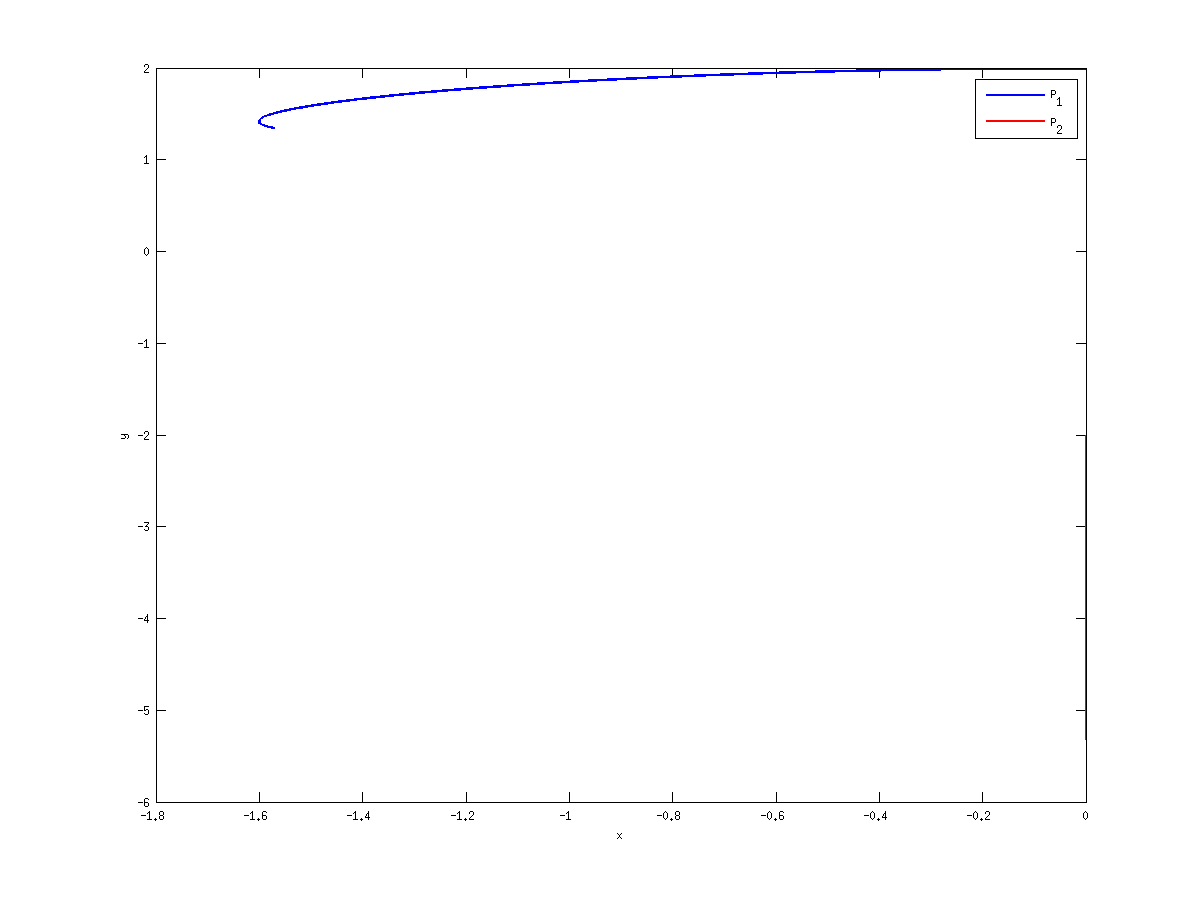
\includegraphics[width=\textwidth]{images/Q2_symplectique2_p.png}
    \caption{$p$ pour symplectique2}
    \label{fig:q2_symplectique2_p}
  \end{subfigure}
  ~
  \begin{subfigure}[b]{0.3\textwidth}
    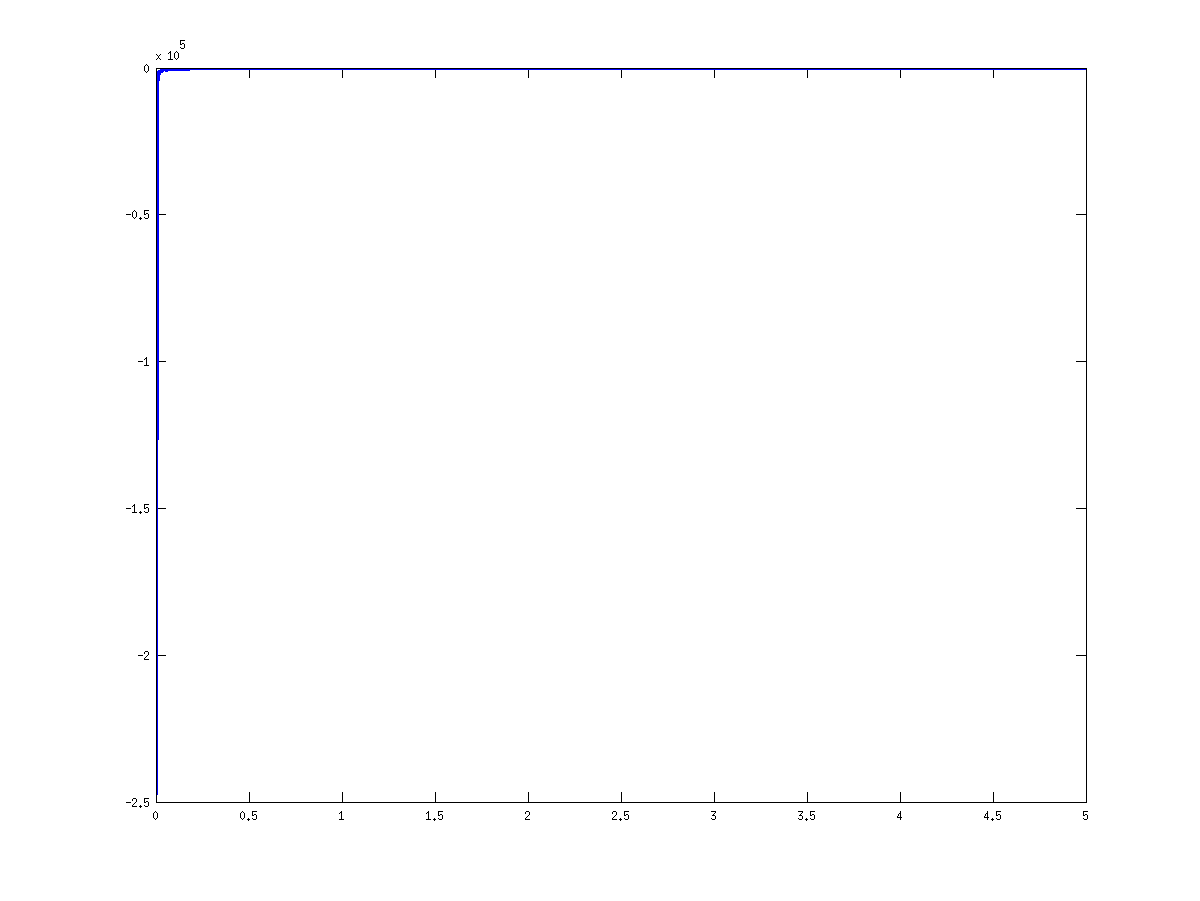
\includegraphics[width=\textwidth]{images/Q2_symplectique2_H.png}
    \caption{$\Ha$ pour symplectique2}
    \label{fig:q2_symplectique2_H}
  \end{subfigure}
  \caption{Résultats pour la question 2}\label{fig:q2}
\end{figure}
